\section{Δένδρα Merkle} \label{section:2-3-merkle-trees}

Ένα δένδρο Merkle (Merkle tree ή hash tree) είναι μία δενδρική δομή δεδομένων, η οποία απαρτίζεται από φύλλα (leaf nodes), που περιέχουν hashes από blocks δεδομένων, και από άλλους κόμβους (non-leaf nodes), οι οποίοι περιέχουν τα hashes των θυγατρικών τους. Στην κορυφή του δένδρου βρίσκεται ο ριζικός κόμβος με το λεγόμενο root hash.\cite{2.3-merkle-tree}

Η πιο συνηθισμένη υλοποίηση είναι το δυαδικό (binary) δένδρο Merkle, το οποίο περιλαμβάνει δύο θυγατρικούς κόμβους (child nodes) κάτω από κάθε γονικό non-leaf κόμβο, και είναι αυτό που αναλύεται στη συνέχεια.

\begin{figure}[H]
	\centering
	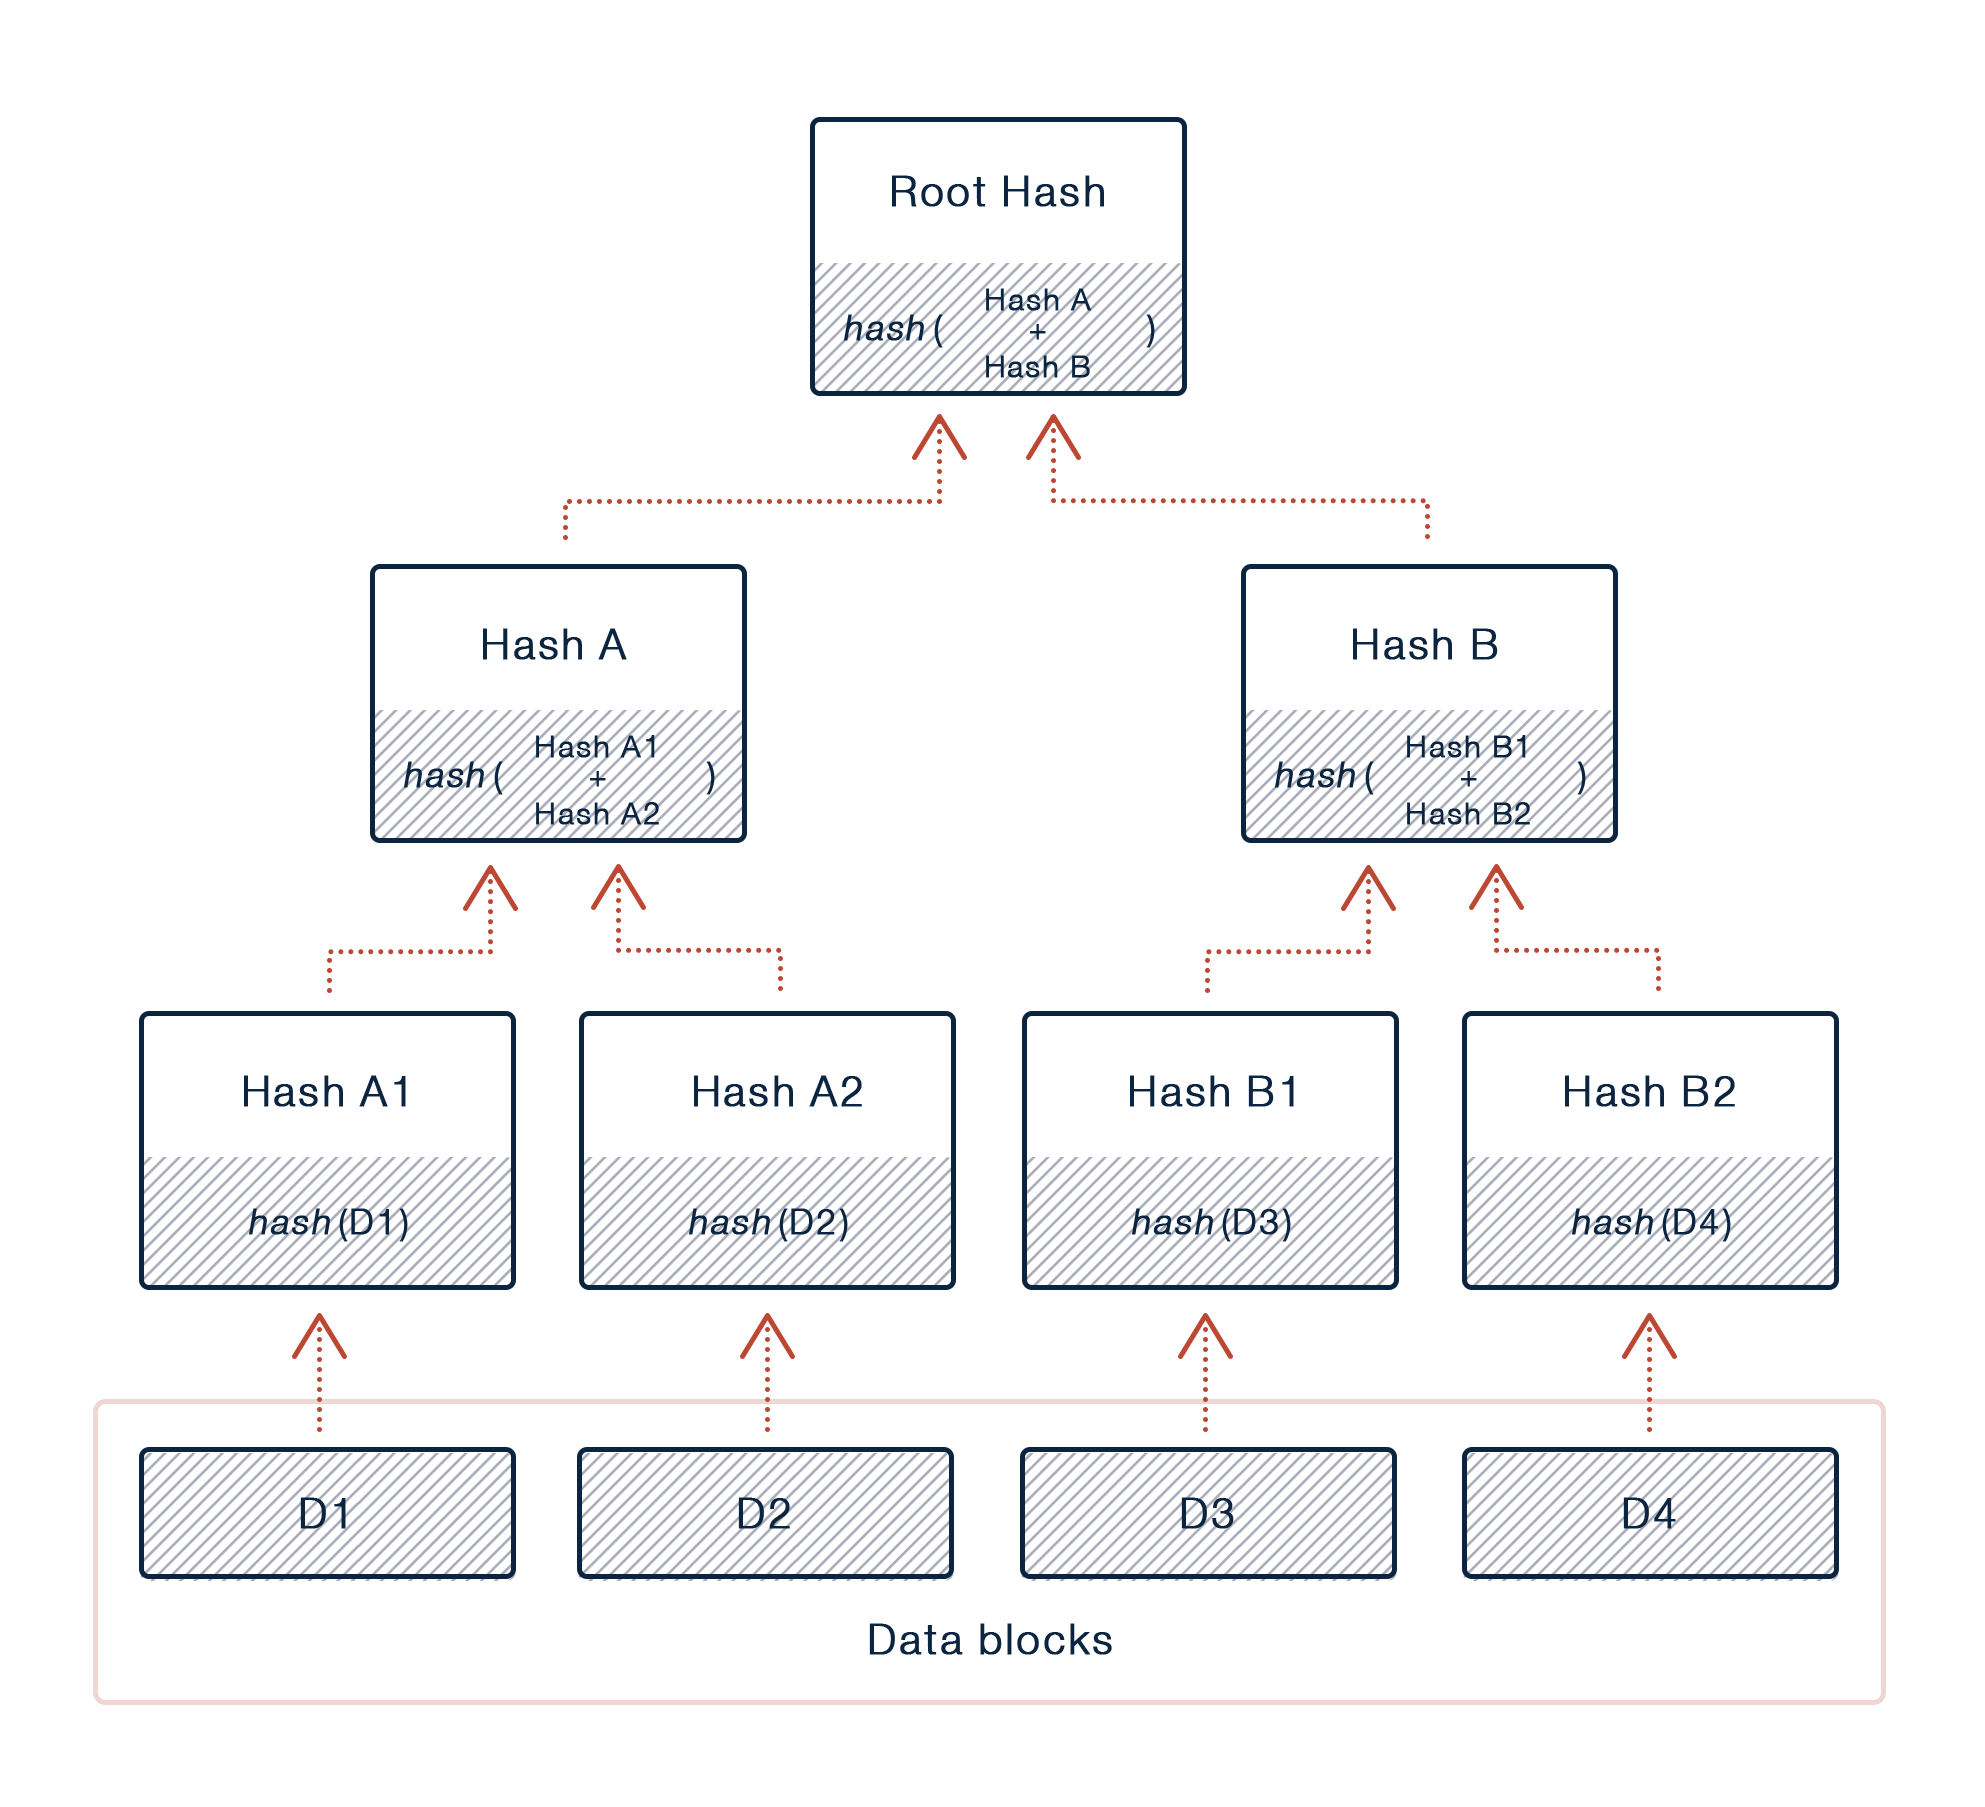
\includegraphics[width=.95\textwidth]{assets/figures/chapter-2/2.3.merkle-tree.png}
	\caption{Παράδειγμα δυαδικού δένδρου Merkle}
\end{figure}

Τα Merkle trees επιτρέπουν την αποδοτική και ασφαλή επαλήθευση των περιεχομένων που ανήκουν σε σετ δεδομένων μεγάλου μεγέθους. Η βασική ιδιότητα είναι ότι για κάθε σετ δεδομένων υπάρχει ακριβώς ένα πιθανό δένδρο, το οποίο δε γίνεται να τροποποιηθεί χωρίς να αλλάξει ταυτόχρονα και το root hash. 

Έτσι, μέσω των λεγόμενων Merkle proofs, μπορούμε:
\begin{itemize}
	\item Να αποφανθούμε εάν κάποια δεδομένα ανήκουν στο δένδρο (με τον αριθμό των hashes που θα πρέπει να υπολογιστούν να είναι ανάλογος του λογαρίθμου του αριθμού των leaf nodes).
	\item Να αποδείξουμε συνοπτικά την εγκυρότητα ενός τμήματος κάποιου σετ δεδομένων, χωρίς να χρειαστεί να αποθηκεύσουμε ολόκληρο το σύνολο δεδομένων.
	\item Να διασφαλίσουμε την εγκυρότητα ενός συγκεκριμένου συνόλου δεδομένων εντός ενός μεγαλύτερου σύνολου, χωρίς να χρειαστεί να αποκαλυφθεί το περιεχόμενο οποιουδήποτε εκ των δύο.\cite{2.3-merkle-proofs-explained} 
\end{itemize}
